\documentstyle[12pt,epsfig]{article}
\setlength{\unitlength}{1.cm}
\doublerulesep -1pt 
\textwidth=6.5in 
\textheight=9in
\hoffset=-1cm 
\voffset=-1in 
\pagestyle{empty}
\begin{document}

\begin{center}
{\bf\sc Massachusetts Institute of Technology}\\
{\bf\sc Experimental Study Group}\\
{\bf\sc 8.022 Spring 2011}\\
\bigskip
{\bf\sc Solution Special relativity}
\end{center}

1.

\newpage

\begin{enumerate}

\item[2] Invariant interval: A quantity that is left unchanged by Lorentz
transformations is a called a ``Lorentz invariant''. Consider two
events described in the laboratory frame by $(t_1, x_1, y_1, z_1)$ and
$(t_2, x_2, y_2, z_2)$. Show that
\begin{equation}
\Delta s^2=-(c\Delta t)^2+(\Delta x)^2+(\Delta y)^2+(\Delta z)^2.
\end{equation}
is a Lorentz invariant.\\

Let's label events 1 and 2 in the laboratory frame
by $(t_1, x_1, y_1, z_1)$ and $(t_2, x_2, 
y_2, z_2)$, and in the boosted frame by
$(t'_1, x'_1, y'_1, z'_1)$ and $(t'_2, x'_2, 
y'_2, z'_2)$.  For simplicity suppose boosted direction is along
positive x-axis and the boost frame is of relative velocity $v$ to the
laboratory frame.  The
transformation law for event 1 reads
\begin{eqnarray}
ct'_1 &=& \gamma (ct_1-\beta x_1)\nonumber\\
x'_1 &=&  \gamma (x_1-\beta ct_1)\nonumber\\
y'_1 &=& y_1\nonumber\\
z'_1 &=& z_1,
\end{eqnarray}
where $\beta=v/c$ and $\gamma=(1-\beta^2)^{-1/2}$.  For event 2 the
transformation is simply to rewrite all subscripts ``1'' in eq.(2) to
subscript ``2''.  The spacetime interval $\Delta s^2$ in boosted frame
then becomes
\begin{eqnarray}
\Delta s'^2 &=& -(c\Delta t')^2+(\Delta x')^2+(\Delta y')^2+(\Delta
z')^2\nonumber\\
&=&-(ct'_2-ct'_1)^2+(x'_2-x'_1)^2+(y'_2-y'_1)^2+(z'_2-z'_1)^2\nonumber\\
&=&-\gamma^2[(ct_2-ct_1)-\beta(x_2-x_1)]^2+\gamma^2[(x_2-x_1)-\beta
(ct_2-ct_1)]^2\nonumber\\
&&+(y_2-y_1)^2+(z_2-z_1)^2\nonumber\\
&=&-\gamma^2(1-\beta^2)(ct_2-ct_1)^2+\gamma^2(1-\beta^2)(x_2-x_1)^2
+(y_2-y_1)^2+(z_2-z_1)^2\nonumber\\
&=& -(c\Delta t)^2+(\Delta x)^2+(\Delta y)^2+(\Delta z)^2\nonumber\\
&=& \Delta s^2.
\end{eqnarray}
So $\Delta s^2$ is a Lorentz invariant.

\newpage

\item[3] Galilean tranformations: Prior to special relativity, 
people related coordinates between different frames 
with the ``Galilean transformation'' -- clocks in different 
reference frame tick at the same rate, spatial positions 
are shifted by a term that depends on the relative velocity 
just as you would expect. For example, for frames that are 
moving with respect to each other in the x direction, we would have
\begin{eqnarray}
t' &=& t\nonumber\\
x' &=& x-vt
\end{eqnarray}
Using the binomial expansion on $\gamma$, show that for 
small $v/c$ the Lorentz tranformations reduce to the Galilean 
tranformations. At what value of $v$ does the next term 
in the expansion change the $x$ transformation by 1\%?\\

The Lorentz transformation reads in eq.(2) without subscripts ``1''
for the sake of generality.  Note that as $\beta=v/c\ll 1$, 
\begin{equation}
\gamma=(1-\beta^2)^{-1/2}\simeq 1+\frac{1}{2}\beta^2+\cdots,
\end{equation}
where ``$\cdots$'' denotes terms in the order ${\mathcal{O}}(\beta^4)$.
Then Lorentz transformation reduces to be 
\begin{eqnarray}
ct'&=&(ct-\beta x)(1+\frac{1}{2}\beta^2)=ct+\mathcal{O}(\beta);\nonumber\\
x'&=& (x-\beta ct)(1+\frac{1}{2}\beta^2)=x-vt+{\mathcal{O}}(\beta^2).
\end{eqnarray}
or $t'=t$, $x'=x-vt$.  This is exactly Galilean transformation.  The
next term in the expansion of $x$ transformation is $(1/2)x\beta^2$,
so it changes by a rate $((1/2)x\beta^2)/x=(1/2)\beta^2=1\%$.  This gives
$v=0.14c\simeq 4\times 10^7 m/s$, beyond which, that means, the
relativistic effect cannot be ignored and Newton Mechanics is not quite
valid anymore.

\newpage

\item[4] Transforming velocities: A bullet is fired with velocity 
$\vec{u'}$ in the $(x', y')$ plane of a moving frame $F'$. 
Frame $F'$ moves with speed $v$ in the $+x$ direction 
with respect to the laboratory frame $F$.\\

(a) Find the angle that the velocity vector makes 
with x axis of the lab frame.\\

The velocity transforms as
\begin{eqnarray}
u_x &=& \frac{u'_x+v}{1+\frac{vu'_x}{c^2}}\\
\vec{u}_{\bot} &=& \frac{\vec{u'}_{\bot}}{\gamma_v (1+\frac{vu'_x}{c^2})},
\end{eqnarray}
where $\gamma_v=(1-v^2/c^2)^{-1/2}$; $u_x$ and $\vec{u}_{\bot}$ are
respectively the component of velocity $\vec{u}$ in lab frame $F$ in x
direction and in the direction normal to x.  Similar notations with
primes are for velocity $\vec{u'}$ in moving frame $F'$.  Let the
angle that $\vec{u}$ makes with respect to $x$-axis in $F$ be
$\theta$, and that $\vec{u'}$ makes with respect to $x'$-axis in $F'$
be $\theta '$.  So $u_x=u\cos{\theta}$,
$|\vec{u}_{\bot}|=u\sin{\theta}$, and similarly for $u'_x$ and
$\vec{u'}_{\bot}$.  Let $u=|\vec{u}|$, and $u'=|\vec{u'}|$.
\begin{eqnarray}
\tan{\theta} &=& \frac{|\vec{u}_{\bot}|}{u_x}= \frac{u'\sin{\theta'}}
{\gamma_v(u'\cos{\theta'}+v)}\\
u &=& \sqrt{u_x^2+|\vec{u}_{\bot}|^2}=
\frac{\sqrt{u'^2+v^2+2u'v\cos{\theta'}-(u'v\sin{\theta'}/c)^2}}
{1+\frac{u'v}{c^2}\cos{\theta'}}.
\end{eqnarray}
(Eq.(10) is for the use of part (c).)  Or for our problem,
\[\theta=\arctan{\left(\frac{u'\sin{\theta'}}
{\gamma_v(u'\cos{\theta'}+v)}\right)}.\]

(b) What is this angle in the limit $|\vec{u'}|=c$? Does anything
wierd happen?\\

Plug in $u'=c$ to eq.(9).
\begin{equation}
\tan{\theta}=\frac{\tan{\theta'}}{\gamma_v (1+\frac{v}{c}\sec{\theta'})}.
\end{equation}
We observe that $\theta'\neq\theta$ generically except when
$v\rightarrow 0$ or $\theta'=0$.  This means that observers in
different frame will observe different orientation of light if their
relative velocity is not in the same direction of the emitted light.
Nothing particularly wierd happens --- we just get a slightly simpler
version of the formula.\\

(c) Show that when $|\vec{u'}|=c$, $|\vec{u}|=c$ -- the 
speed of light is the same in both frames.\\

Plugging $u'=c$ to eq.(10):
\begin{eqnarray*}
u &=& \frac{\sqrt{c^2+v^2+2cv\cos{\theta'}-v^2\sin^2\theta'}}
{1+v\cos{\theta'}/c}
\\
&=& \frac{\sqrt{c^2+2cv\cos\theta'+v^2(1 - \sin^2\theta')}}
{1+v\cos{\theta'}/c}
\\
&=& \frac{\sqrt{c^2+2cv\cos\theta'+v^2\cos^2\theta'}}
{1+v\cos{\theta'}/c}
\\
&=& \frac{\sqrt{(c + v\cos\theta')^2}}{1+v\cos{\theta'}/c}
\\
&=& \frac{c + v\cos\theta'}{1+v\cos{\theta'}/c} = c\;.
\end{eqnarray*}

\newpage

\item[5] ``Beating the speed of light'': ... The idea is as follows.  We
make a cart roll across the floor with speed $v$.  We put a smaller
cart on top of that cart, and roll it with speed $v$ with respect to
the first cart, and in the same direction as the first cart. We put a
third cart on this second cart; it rolls with speed $v$ with respect
to the second cart. We put a fourth cart ... you get the idea.  Your
uncle claims that there is some $n$ at which the cart must be going
faster than the speed of light.\\ (a) Prove him wrong. Using
mathematical induction, prove that if $v < c$, then $v_n < c$, where
$v_n$ is the velocity of the $n$th cart. Show that this holds even for
extremely large $n$.\\

Eq.(7) gives the recurrence relation of $v_{n+1}$ (the $(n+1)$th
cart's velocity with respect to the floor) in terms of $v_n$ and $v$,
i.e. we think of the floor as the lab frame and $n$th cart as the
moving frame with boost velocity $v_n$; the ($n+1$)th cart moves with
velocity $v$ with repect to the $n$th cart.  (When you apply eq.(7),
be careful of the meaning of notations since $v$ in eq.(7) means boost
velocity.) The recurrence relation is
\begin{equation}
v_{n+1}=\frac{v+v_n}{1+v\,v_n/c^2}.
\end{equation}
Now let's prove by induction that, assuming $v<c$, then $v_n<c$ for all $n$.  
Firstly we observe that $v_1=v<c$ by assumption.
Then, suppose $v_n<c$ holds, show that $v_{n+1}<c$ :  let $\beta_v=v/c$,
$\beta_n=v_n/c$, and so on.
\begin{eqnarray}
\beta_{n+1}^2 = (\frac{v_{n+1}}{c})^2 &=& \left(\frac{\beta_v+\beta_n}{1+\beta_v
\beta_n}\right)^2\nonumber\\
&=& 1-\frac{(1-\beta_v^2)(1-\beta_n^2)}{(1+\beta_v
\beta_n)^2}\nonumber\\
&<& 1.
\end{eqnarray}
Therefore, by mathematical induction we deduce that $v_n<c$ for {\sl all}
$n$ if $v<c$, including for extremely large $n$.\\

(b) Calculate the value of $v_n$ given $v$ and $n$. \\

Define $\beta_n=v_n/c=\tanh{(x_n)}$; so
$\beta_v=v/c=v_1/c=\tanh{(x_1)}$.
\begin{eqnarray}
\tanh{(x_{n+1})}&=&\frac{\tanh{(x_1)}+\tanh{(x_n)}}{1+\tanh{(x_1)}\tanh{(x_n)}}
\nonumber\\
&=& \tanh{(x_1+x_n)}.
\end{eqnarray}
Since $\tanh{(x)}$ is a monotonically increasing function, the 
recurrence relation simplifies to be $x_n=x_{n-1}+x_1$ for
$n\ge 2$.  This gives 
\begin{eqnarray}
x_n &=& nx_1\\
v_n &=& c\tanh{(nx_1)}=c\tanh{(n\,{\rm arctanh}(v/c))}.
\end{eqnarray}
As $n\rightarrow\infty$, $x_n\rightarrow\infty$,
$\tanh{(x_n)}\rightarrow 1$.  In other words, $v$ limits to the speed
of light, but never beats it.

\item[6] Energy-momentum identity.

Start from the fact that $E=\gamma_u mc^2$, $\vec{p}=\gamma_u
m\vec{u}$ where $\gamma_u=(1-u^2/c^2)^{-1/2}$.
\begin{eqnarray}
p^2 c^2+m^2 c^4 &=& m^2 c^4 (1+\frac{\gamma_u^2 u^2}{c^2})\nonumber\\
&=& m^2 c^4 (1+\frac{u^2/c^2}{1-u^2/c^2})\nonumber\\
&=& \gamma_u^2 m^2 c^4\nonumber\\
&=& E^2.
\end{eqnarray}


\newpage

\item[7] Transformation of fields: A very large sheet of charge 
lies in the $x-y$ plane of the frame $F$. The charge per 
unit area of this sheet is $\sigma$. In the frame $F'$, 
this sheet moves to the right with speed $v$.

\begin{figure}[ht]
\begin{center}
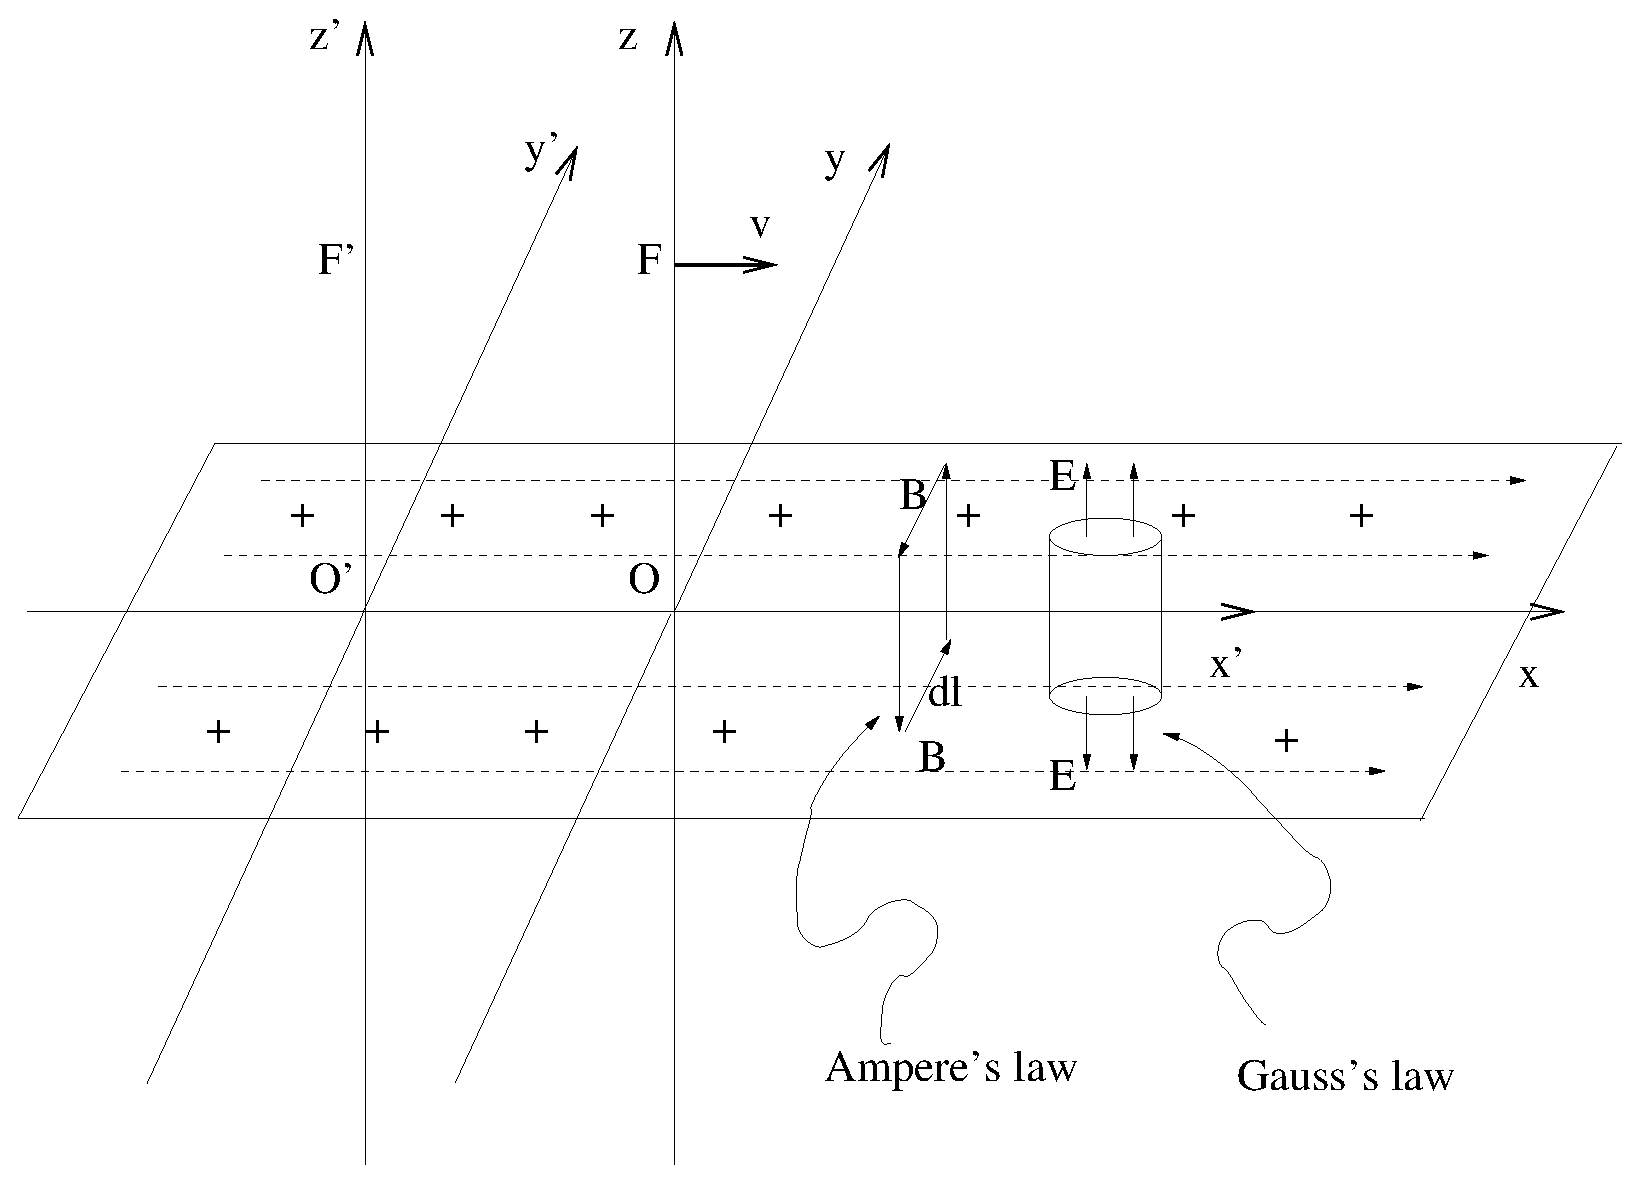
\epsfig{file = fields10.eps, width = 11cm}
\label{fig:fields10}
\caption{A sheet of charge of density $\sigma$ stays at rest in frame
$F$, and moves with velocity $v$ along positive x-axis in frame $F'$.
It has density $\sigma'=\gamma\sigma$ in $F'$.}
\end{center}
\end{figure}

(a) What is the electric field in the rest frame (above and below the
sheet)?\\

Refer to figure 1.  In rest frame $F$, we just apply Gauss's law.  
\begin{eqnarray}
2EA &=& 4\pi\sigma A,\\
E &=& 2\pi\sigma.
\end{eqnarray}
Note that the direction of $\vec{E}$ is upward in $z>0$ and downward
in $z<0$ (if we assume the charge is positive).  So 
\begin{equation}
\vec{E}=2\pi\sigma\:Sign(z)\hat z,
\end{equation}
where $Sign(z)=1,\;z>0;\;-1,\;z<0$.\\

(b) What is the electric field in the frame $F'$ (above and below the
sheet)?\\

We shall follow the same derivation as in part (a).  But be careful of
the charge density.  If the sheet moves in positive x-axis,
$dx'=dx/\gamma,\;dy'=dy$, so $\sigma'=\gamma\sigma$, where
$\gamma=(1-v^2/c^2)^{-1/2}$.  So we have
\begin{equation}
\vec{E'}=2\pi\sigma'\:Sign(z)\hat z=2\pi\gamma\sigma\:Sign(z)\hat z.
\end{equation}

(c) What is the magnetic field in the frame $F'$ (above and below the
sheet)?\\

The current on the sheet (due to the moving of the charge) {\sl per
unit length} is $dI/dl=\sigma' v$ in frame $F'$, where $dl$ is a
length normal to the current flow.  You can achieve this result by
considering that during a time $dt$, some charges of 
an area of $vdt\,dl$ cross the line $dl$.  Due to the symmetry, the
magnetic field at $z>0$ is along negative y-axis, and at $z<0$ along
positive y-axis, so that the circulation of  the loop in Figure 1 
observes right-hand rule with the direction of current flow.  Apply
Ampere's law:
\begin{eqnarray}
2B'dl&=&\frac{4\pi}{c}\sigma'vdl,\\
B'&=&\frac{2\pi}{c}\sigma' v=\frac{2\pi}{c}\gamma\sigma v.
\end{eqnarray}
Considering the direction,
\begin{equation}
\vec{B'}=-\frac{2\pi}{c}\gamma\sigma v\,Sign(z)\hat{y}.
\end{equation}

(d) Show that the results of (b) and (c) are consistent with 
the general Lorentz transformations for electric and magnetic fields, 
Eq. (60) of Purcell Chapter 6.\\

A little caution is that in eq.(60) of Purcell, $F$ moves in negative
x-axis seen from $F'$; so we should change $\beta\rightarrow -\beta$
in eq.(60).  
\begin{eqnarray}
E'_{\|}&=&E_{\|}=0;\\
\vec{E'}_{\bot}&=&\vec{E'}=2\pi\gamma\sigma\:Sign(z)\hat{z}\nonumber\\
&=&\gamma\vec{E}=\gamma(\vec{E}_{\bot}-\vec{\beta}\times\vec{B}_{\bot});\\
B'_{\|}&=&B_{\|}=0;\\
\vec{B'}_{\bot}&=&\vec{B'}= -\frac{2\pi}{c}\gamma\sigma v\,Sign(z)\hat{y}
\nonumber\\
&=& \gamma(\vec{B}_{\bot}+\vec{\beta}\times \vec{E}_{\bot}).
\end{eqnarray}
Note that $\vec{B}=0$ and $\vec{E}=\vec{E}_{\bot}$ in frame $F$, 
$\vec{\beta}=\beta\hat{x}$, $\hat{x}\times\hat{z}=-\hat{y}$.

\end{enumerate}
\end{document}
